\documentclass[30pt]{article}
\usepackage[space,fancyhdr,fntef]{ctexcap}
\usepackage{fontspec}
\fontspec{宋体}
\setmainfont{Times New Roman}
%\fontsize{50pt}{50pt}\selectfont
\renewcommand{\rmdefault}{ptm}
\usepackage[namelimits,sumlimits,nointlimits]{amsmath}
\usepackage[bottom=20mm,top=30mm,left=25mm,right=25mm,centering]{geometry}
\usepackage{color}
\usepackage{CJKfntef}%下划线宏包160页
\usepackage{xcolor}
\usepackage{arydshln}%234页,虚线表格宏包
\pagestyle{fancy} \fancyhf{}
\fancyhead[OL]{\color{gray}~~~班序号:Java41班 \hfill 姓名:王松年~~~}
\fancyfoot[C]{\color{gray}\thepage}
%\renewcommand{\footrulewidth}{0.4pt}%改为0pt即可去掉页脚上面的横线
%\usepackage{parskip}
%\usepackage{indentfirst}
\usepackage{graphicx}%插图宏包,参见手册318页
\definecolor{dkgreen}{RGB}{106,135,89}
\definecolor{dkblue}{RGB}{103,150,163}
\definecolor{wgray}{RGB}{248,248,248}

\usepackage{multirow}%跨行表格宏包216页
\usepackage{array}%数组宏包209页

\usepackage{listings}
\lstset{language=Java,
backgroundcolor=\color{wgray},
rulesepcolor=\color{red!20!green!20!blue!20},%代码块边框为淡青色
%lablestep=1,
%lablesep=5pt,
%lablestyle=\tiny,
%tablesize=4,
%captionpos=b,
basicstyle=\ttfamily\small,
keywordstyle=\color{orange},
commentstyle=\color{gray},
stringstyle=\color{dkgreen},
numberstyle=\tiny,
numbersep=8pt,
frame=single,%topline.bottomline,lines,single,leftline
identifierstyle=\color{dkblue},
numbers=left,
stepnumber=1,
xleftmargin=2em,xrightmargin=2em, aboveskip=1em,
breaklines=true,
showstringspaces=true
}
\usepackage[xetex,colorlinks]{hyperref}%394页  \href{网址}{文本}
\hypersetup{urlcolor=blue}
%\linebreak[2]%换行,152页
\usepackage{fancybox}%盒子宏包55页

\begin{document}
\flushbottom
\newcommand{\dm}[1]{\colorbox{wgray}{\lstinline^#1^}}
\newcommand{\myroman}[1]{\uppercase\expandafter{\romannumeral#1}}
\newcounter{num}[section] \renewcommand{\thenum}{\arabic{num}.} \newcommand{\num}{\refstepcounter{num}\text{\thenum}}
%\newlength{\mylen}
%\settowidth{\mylen}{Tips}
%\settoheight{\myheight}{T}
\newenvironment{tips}{\kaishu\zihao{-6}\color{blue}{\noindent\rule[-3pt]{\textwidth}{0.5pt}\par \em \noindent {\zihao{-5} \textcolor[rgb]{1.00,0.00,0.00}{Tips}}}\par}{\\ \rule[3mm]{\textwidth}{0.5pt}\par}

\newenvironment{jie}{\kaishu\zihao{-5}\color{blue}{\noindent\em 解:}\par}{\hfill $\diamondsuit$\par}

%\begin{lstlisting}
%1
%\end{lstlisting}

%
%\newlength{\mylen}
%\settowidth{\mylen}{For iasasasaasasaasdadadsadasd =10}
%\makebox[0pt][l]%55页
%{
%\color{wgray}\rule[0pt]{\mylen}{5pt}%59页
%}


%\lstinline[参数]符号 源程序 符号。
\CTEXsetup[name={Day~,}]{section}

%\href{https://www.baidu.com/?tn=40020637_11_oem_dg}{百度}

%\rule[1.3mm]{1cm}{1pt}tips\rule[2.5mm]{1cm}{1pt}
%
%
%\begin{tips}
%123
%\end{tips}


\section{}%day1
\num 如果\dm{int x=20, y=5},则语句\dm{System.out.println(x+y + "" +(x+y)+y);}的输出结果是(~~~\textcolor[rgb]{1.00,0.00,0.00}{D}~~~)。

A.\dm{2530} \hspace{2.5cm} B.\dm{55} \hspace{2.5cm} C.\dm{2052055}\hspace{2.5cm} D.\dm{25255}

\begin{jie}
先计算\dm{()}里的:x + y = 25.

从左向右计算:\dm{x + y} 为\dm{25},遇到字符串将数字转为字符串,然后将后边的续接到前边:25255.
\end{jie}

\num 在Java中,在同一包内,类Cat里面有个公共方法sleep(),该方法前有static修饰,则可以直接用Cat.sleep()。(~~~\textcolor[rgb]{1.00,0.00,0.00}{A}~~~)

A.\dm{正确} \hspace{2.5cm} B.\dm{错误} \hfill \hphantom{C.\dm{205255}}\hfill\hphantom{D.\dm{25255}}\hfill \hphantom{~}

\begin{tips}
用\dm{static}修饰的为类方法,类方法可由类名直接调用。
\end{tips}

\num 给定以下方法声明,调用执行\dm{mystery(1234)}的输出结果是(~~~\textcolor[rgb]{1.00,0.00,0.00}{B}~~~)。

\begin{lstlisting}
//precondition: x >= 0
public void mystery (int x) {
    System.out.print(x % 10);
    if ((x / 10) != 0){
        mystery(x / 10);
    }
    System.out.print(x % 10);
}
\end{lstlisting}

A.\dm{1441} \hspace{2.42cm} B.\dm{43211234} \hspace{1.5cm} C.\dm{3443}\hspace{3cm} D.\dm{12344321}

\begin{jie}
x\%10 = 1234 \% 10 = \textcolor[rgb]{1.00,0.00,0.00}{4}
\end{jie}
\begin{tips}
该方法的第3$\sim$6行的功能是实现逆序打印。
\end{tips}

\num 实现函数\dm{ToLowerCase()},该函数接收一个字符串参数\dm{str},并将该字符串中的大写字母转换成小写字母,之后返回新的字符串。\href{https://leetcode-cn.com/problems/to-lower-case/\%20--with-chrome-plus-plus\%20--disable-features=RendererCodeIntegrity,FlashDeprecationWarning/}{OJ链接-转换成小写字母}

\begin{lstlisting}[title= 转换成小写字母]
class Solution {
    public String toLowerCase(String str) {
        return str.toLowerCase();
    }
}
\end{lstlisting}

\begin{tips}
转大写:\dm{str.toUpperCase()}

转小写:\dm{str.toLowerCase()}
\end{tips}

\num 给定一个数组,将数组中的元素向右移动k个位置,其中k是非负数。\href{https://leetcode-cn.com/problems/rotate-array/\%20--with-chrome-plus-plus\%20--disable-features=RendererCodeIntegrity,FlashDeprecationWarning/} {OJ链接-旋转数组}

\begin{lstlisting}[title = 旋转数组]
class Solution {
    public void rotate(int[] nums, int k) {
        k %= nums.length;
        reverse(nums,0,nums.length-1);
        reverse(nums,0,k-1);
        reverse(nums,k,nums.length-1);

    }
    public void reverse(int[] nums,int lo,int hi){
        while(lo < hi){
            int tmp = nums[lo];
            nums[lo] = nums[hi];
            nums[hi] = tmp;
            lo++;
            hi--;
        }
    }
}
\end{lstlisting}

\begin{tips}
在C语言做过这个题。

1.要先把旋转的位置除数组的长度取余,因为向右移动数组长度个位置(或其倍数)等于没有移动。

2.把整个数组旋转得到新的数组。

3.依次旋转数组的前\dm{k}个元素(\dm{0到k-1}),和后边剩余的元素。
\end{tips}
\newpage
\section{}%day2
\num 如果类的方法没有返回值,该方法的返回类型是(~~~\textcolor[rgb]{1.00,0.00,0.00}{A}~~~)。

A.\dm{void}\hfill B.\dm{null} \hfill C.\dm{abstract}\hfill D.\dm{default}

\num \dm{Java Application(Java应用程序)}源程序文件编译后的字节码文件的拓展名是(~~~\textcolor[rgb]{1.00,0.00,0.00}{B}~~~)。

A.\dm{java}\hfill B.\dm{class}\hfill C.\dm{exe}\hfill D.\dm{jar}

\begin{tips}
Java源文件的拓展名:\dm{java}

Java源文件编译后拓展名:\dm{class}
\end{tips}

\num 关于继承的描述正确的是(~~~\textcolor[rgb]{1.00,0.00,0.00}{C}~~~)。

A.函数的出口应该尽可能少,最好只有一个出口

B.为了防止程序中的内存泄漏,应该不使用动态内存分配

C.在函数实现中应该少使用全局变量

D.函数的功能应该单一

\begin{tips}
A.函数应为每个逻辑分支提供出口。

B.动态内存分配无法避免,应该及时回收空间和释放指针避免动态内存泄露。

C.为保证封装性,尽量少用全局变量。

D.函数可以根据不同的输入来实现相应的功能(重载)。
\end{tips}

\num 给定一个数组\dm{nums}和一个值\dm{val},你需要原地移除所有数值等于\dm{val}的元素,返回移除后数组的新长度。不要使用额外的数组空间,你必须在原地修改输入数组并在使用$O(1)$额外空间的条件下完成。\href{https://leetcode-cn.com/problems/remove-element/\%20--with-chrome-plus-plus\%20--disable-features=RendererCodeIntegrity,FlashDeprecationWarning/} {OJ链接-移除元素}

\begin{tips}
1.边界情况:数组为空时,要返回0。

分析:不考虑顺序,返回的为不含\dm{val}的前边一段,思路:把\dm{val}换到后边去。

2.左指针\dm{lo}指向数组的左边,找\dm{val},如果没找到\dm{val},就把这个指针向右移动;

3.右指针\dm{hi}指向数组的右边,\dm{val}就应该位于数组后边,所以如果值是\dm{val},指针就左移。

4.经过2、3步后,左指针指的是\dm{val},右指针指的是非\dm{val},将这俩指针对应元素交换。

5.左右指针重合时,数组就遍历完了。

6.左指针的左边一定是不含\dm{val}的,其左边有\dm{lo}个元素,如果此时的左指针对应元素的值时\dm{val},那就返回\dm{lo},如果左指针对应元素的值不是\dm{lo},就返回\dm{lo + 1}。
\end{tips}

\begin{lstlisting}[title = 移除元素]
class Solution {
    public int removeElement(int[] nums, int val) {
        if(nums.length == 0){
            return 0;
        }
        int lo = 0;
        int hi = nums.length - 1;
        int len = 0;
        while(lo < hi){
            if(nums[lo] != val && lo < hi){
                lo++;
            }
            if(nums[hi] == val && lo < hi){
                hi--;
            }
            if(lo < hi){
                int tmp = nums[lo];
                nums[lo] = nums[hi];
                nums[hi] = tmp;
            }
        }
        if(nums[lo] == val){
            return lo;
        }
        return lo + 1;
    }
}
\end{lstlisting}

\num 给定一个排序数组和一个目标值,在数组中找到目标值,并返回其索引。如果目标值不存在于数组中,返回它将会被按顺序插入的位置,你可以假设数组中无重复元素。\href{https://leetcode-cn.com/problems/search-insert-position/\%20--with-chrome-plus-plus\%20--disable-features=RendererCodeIntegrity,FlashDeprecationWarning/} {OJ链接-搜索插入位置}

\begin{tips}
有序数组,采用二分查找。

1.找到元素:返回元素的下标。

2.如果数组中没有该元素。退出循环的前一次左指针、右指针、中间指针指向同一元素,若该元素小于目标值,即\dm{nums[mid] < target},左指针指向中间指针的下一个元素,此时左指针在右指针的右边,退出循环。同时左指针指向的位置也是目标元素要插入的位置。

3.若该元素大于目标值,即\dm{target < nums[mid]},右指针指向中间指针的前一个元素,右指针在左指针的左边,退出循环。左指针的左侧元素必定小于目标值,而左指针指向的元素大于目标值,目标值应该插入到左指针指向的位置处。

4.综上,找到目标值就返回该目标值对应的下标,没找到该目标值就返回左指针指向的位置。
\end{tips}

\begin{lstlisting}[title = 搜索插入位置]
class Solution {
    public int searchInsert(int[] nums, int target) {
        if(nums.length == 0){
            return 0;
        }
        int lo = 0;
        int hi = nums.length - 1;
        int mid = (lo + hi)/2;
        while(lo <= hi){
            mid = (lo + hi)/2;
            if(nums[mid] < target){
                lo = mid + 1;
            }else if(target < nums[mid]){
                hi = mid - 1;
            }else{
                return mid;
            }
        }
        return lo;
    }
}
\end{lstlisting}

\newpage
\section{}%day3
\num 以下代码的循环次数是(~~~\textcolor[rgb]{1.00,0.00,0.00}{D}~~~)。

\begin{lstlisting}[numbers=none]
public class Test {
    public static void main(String[] args) {
        int i = 7;
        do {
            System.out.println(--i);
            --i;
        } while (i != 0);
        System.out.println(i);
    }
}
\end{lstlisting}

A.\dm{0}\hfill B.\dm{1}\hfill C.\dm{7}\hfill D.\dm{无限次}

\begin{jie}
\dm{i}的初始值为奇数,循环中每次减2,退出条件为不等于0,奇数减2永远不会为0,即死循环。
\end{jie}

\num 下列选项中属于面向对象设计方法的主要特征是(~~~\textcolor[rgb]{1.00,0.00,0.00}{A}~~~)。

A.继承\hfill B.自顶向下\hfill C.模块化\hfill D.逐步求精

\begin{tips}
面向对象最主要的几个特征:封装、继承、多态、抽象等。
\end{tips}

\num 下面的方法,当输入为$2$的时候返回值是多少(~~~\textcolor[rgb]{1.00,0.00,0.00}{D}~~~)。

\begin{lstlisting}[numbers=none]
public static int getValue(int i) {
    int result = 0;
    switch (i) {
        case 1:
            result = result + i;
        case 2:
            result = result + i * 2;
        case 3:
            result = result + i * 3;
    }
    return result;
}
\end{lstlisting}

A.\dm{0}\hfill B.\dm{2}\hfill C.\dm{4}\hfill D.\dm{10}

\begin{jie}
\dm{case}后没有\dm{break},会继续执行后面的\dm{case},所以结果为:$i\times2 + i\times3 = i\times5 = 2\times5 = 10$
\end{jie}

\num 赎金信。\href{https://leetcode-cn.com/problems/ransom-note/} {OJ链接-赎金信}

给定一个赎金信 (\dm{ransom}) 字符串和一个杂志(\dm{magazine})字符串,判断第一个字符串\dm{ransom}能不能由第二个字符串\dm{magazines}里面的字符构成。如果可以构成,返回\dm{true};否则返回\dm{false}。

(题目说明:为了不暴露赎金信字迹,要从杂志上搜索各个需要的字母,组成单词来表达意思。杂志字符串中的每个字符只能在赎金信字符串中使用一次。)

假设两个字符串均只含有小写字母。

\begin{tips}
1.杂志字符串长度小于赎金信字符串长度,一定不能构成赎金信。

2.因为只有小写字母,所以分别统计各字符的个数,将两字符串各字符的个数放入数组中。

3.分别比较两字符串对应字符的个数,赎金信相应字符的个数超过杂志该字符的个数,则一定不能表示,否则就能表示。
\end{tips}

\begin{lstlisting}[title=赎金信]
class Solution {
    public boolean canConstruct(String ransomNote, String magazine) {
        if(ransomNote.length()>magazine.length()){
            return false;
        }
        char[] ch1 = ransomNote.toCharArray();
        char[] ch2 = magazine.toCharArray();
        int[] rans = new int[26];
        int[] maga = new int[26];
        for(char c1 : ch1){
            rans[c1 - 'a']++;
        }
        for(char c2 : ch2){
            maga[c2 - 'a']++;
        }
        for(int i = 0; i < 26; i++){
            if(rans[i] > maga[i]){
                return false;
            }
        }
        return true;
    }
}
\end{lstlisting}

\num 判断一个整数是否是回文数。回文数是指正序(从左到右)和倒叙(从右向左)读都是一样的整数。\href{https://leetcode-cn.com/problems/palindrome-number/\%20--with-chrome-plus-plus\%20--disable-features=RendererCodeIntegrity,FlashDeprecationWarning/} {OJ链接-回文数}

方法1:

\begin{tips}
1.把数字转为字符串;

2.把字符串转为字符串数组;

3.使用左右指针指向数组的前边和后边,两个指针指向的字符相等指针就同时向中间移动,不相等就退出。

4.左指针小于右指针,不是回文数,否则就是。
\end{tips}

\begin{lstlisting}
class Solution {
    public boolean isPalindrome(int x) {
      String str = "" + x;
      char[] ch1 = str.toCharArray();
      int lo = 0;
      int hi = ch1.length - 1;
      while(lo < hi){
          if(ch1[lo] != ch1 [hi]){
              break;
          }
          lo++;
          hi--;
      }
      if(lo < hi){
          return false;
      }
      return true;
    }
}
\end{lstlisting}

方法2:

\begin{tips}
1.根据题意,所有负数都不是回文数。

2.小于10的自然数都是回文数。

3.能被10整除的都不是回文数。(能被10整除,最后一位是0,而第一位不会是0,所以不是回文数)

4.其他的数字\dm{x},每次从后边取一位\dm{x\%10},放入新的数\dm{num}中:\dm{num = num * 10 + x\%10},

5.每取完一位,就将最后一位拿掉:\dm{x = x / 10}。

判断\dm{x}是不是小于\dm{num},如果小于,说明已经过半了,即:

6.如果\dm{x}是奇数位,例如5位,取了2位后,\dm{x}还有3位,此时\dm{num}是2位,\dm{num < x}。再取一位,\dm{x}变成2位,\dm{num}变成3位,两位数小于三位数,此时说明取的位数超过一半,就不用取了,如果\dm{x}和\dm{num}的前两位\dm{num \ 10}相等,说明是回文数,否则不是。

7.如果\dm{x}是偶数位,例如4位,取了2位后,\dm{num}是2位,\dm{x}剩余2位,如果\dm{num}等于\dm{x},说明是回文数。
\end{tips}

\begin{lstlisting}
class Solution {
    public boolean isPalindrome(int x) {
        if(x < 0){
            return false;
        }
        if(0 <= x && x < 10){
            return true;
        }
        if(x % 10 == 0){
            return false;
        }
        int num = 0;
        while(x > num){
            num = num * 10 + x % 10;
            x /= 10;
        }
        return x == num || x == num / 10;
    }
}
\end{lstlisting}

\newpage
\section{}%day4
\num 下面有关\dm{java final}的基本规则,描述错误的是(~~~\textcolor[rgb]{1.00,0.00,0.00}{B}~~~)。

A.\dm{final}修饰的类不能被继承

B.\dm{final}修饰的成员变量只允许赋值一次,且只能在类方法赋值

C.\dm{final}修饰的局部变量即为常量,只能赋值一次

D.\dm{final}修饰的方法不允许被子类覆盖

\begin{tips}
\dm{final}修饰的类不能被继承,修饰的变量只允许被赋值一次且后边无法改变该变量的值,对于成员变量可以进行就地初始化,也可以进行代码块初始化,也可以使用构造方法初始化,但这三种方法只能使用一个,\dm{final}修饰的方法不支持重写,但是可以进行重载。
\end{tips}

\num 选项中哪一行代码可以替换\dm{//add code here}而不产生编译错误(\hphantom{~~~~~})。

A.\dm{public abstract void method(int a);}

B.\dm{consInt = constInt + 5;}

C.\dm{public int method;}

D.\dm{public abstract void anotherMethod(){}}

\begin{jie}
没有代码,没法做。
\end{jie}

\num 第三行将输出什么(~~~\textcolor[rgb]{1.00,0.00,0.00}{B}~~~)。

\begin{lstlisting}
public class SwitchTest{
    public static void main(String[] args) {
        System.out.println("value=" + switchit(4));
    }
    public static int switchit(int x) {
        int j = 1;
        switch (x) {
            case 1:j++;
            case 2:j++;
            case 3:j++;
            case 4:j++;
            case 5:j++;
            default:j++;
        }
        return j+x;
    }
}
\end{lstlisting}

A.\dm{value=6;}\hfill B.\dm{value=8;}\hfill C.\dm{value=3;}\hfill D.\dm{value=5;}

\begin{jie}
没有遇到\dm{break}会接着往后执行。
\end{jie}

\num 给定一个仅包含大小写字母和空格\dm{' '}的字符串,返回其最后一个单词的长度。如果不存在最后一个单词,请返回0。\href{https://leetcode-cn.com/problems/length-of-last-word/} {OJ链接-最后一个单词的长度}

\begin{tips}
1.字符串长度为0或者字符串引用指向为空,那最后一个单词长度为0.

2.一般情况:

用右指针\dm{hi}从字符串的最后一位开始遍历,如果是空格,指针就向前移动,如果遇到了字母就停下来,记录该位置。当\dm{hi}小于0时,说明字符串遍历完毕也没遇到字母,即不存在最后一个单词,返回0.

如果\dm{hi}不小于0,记录\dm{hi}当前的位置,使用一个新的指针\dm{lo}从该位置向前遍历,直到遇到空格(或遍历字符串结束即\dm{lo}小于0)停下来,\dm{lo}和\dm{hi}之间的字符个数就是最后一个单词的长度。
\end{tips}

\begin{lstlisting}[title=最后一个单词的长度]
class Solution {
    public int lengthOfLastWord(String s) {
        //char[] ch = s.toCharArray();
        int hi = s.length() - 1;
        if(s.length() == 0 || s == null){
            return 0;
        }
        while(hi >= 0 && s.charAt(hi) == ' '){
            hi--;
        }
        if(hi < 0){
            return 0;
        }
        int lo = hi;
        while(lo >= 0 && s.charAt(lo) != ' '){
            lo--;
        }
        return hi - lo;
    }
}
\end{lstlisting}

\num
给你两个有序整数数组 \dm{nums1}和\dm{nums2},请你将\dm{nums2}合并到\dm{nums1}中,使\dm{nums1}成为一个有序数组。\href{https://leetcode-cn.com/problems/merge-sorted-array/} {OJ链接-合并两个有序数组}

\begin{tips}
方法1:将两个数组合并,然后重新排序。

方法2:依据题目描述,此题为归并排序算法的归并部分。

因为最终的结果要存放在\dm{nums1}中,为了避免\dm{nums1}中的数据被覆盖,使用一个数组\dm{arr}来存放\dm{nums1}的数据。

步骤:

1.使用两个指针分别指向数组\dm{arr}和\dm{nums2}的开头,比较其对应元素的大小,将较小的那个元素放入到\dm{nums1}中,同时将\dm{nums1}和拿出元素的那个数组的指针向后移动一位。

2.其中一个数组遍历完后,将没有遍历完的那个数组的剩余部分放在\dm{nums1}后边即可。
\end{tips}

\begin{lstlisting}[title=合并两个有序数组]
class Solution {
    public void merge(int[] nums1, int m, int[] nums2, int n) {
        int[] arr = new int[m];
        for(int i = 0; i < m; i++){
            arr[i] = nums1[i];
        }
        int a1 = 0;
        int a2 = 0;
        int i = 0;
        while(a1 < m && a2 < n){
            if(arr[a1] <= nums2[a2]){
                nums1[i++] = arr[a1++];
            }else{
                nums1[i++] = nums2[a2++];
            }
        }
        for(;i < m + n; i++){
            if(a1 < m){
                nums1[i] = arr[a1++];
            }
            if(a2 < n){
               nums1[i] = nums2[a2++];
            }
        }
    }
}
\end{lstlisting}

\newpage
\section{}%day5
\num 下列Java程序输出的结果为(~~~\textcolor[rgb]{1.00,0.00,0.00}{B}~~~)。
\begin{lstlisting}[numbers=none]
public class Example{
    String str = new String("hello");
    char[] ch = {'a','b'};
    public static void main(String args[]){
        Example ex = new Example();
        ex.change(ex.str, ex.ch);
        System.out.print(ex.str + "and");
        System.out.print(ex.ch);
    }
    public void change(String str,char ch[]){
        str = "test ok";
        ch[0] = 'c';
    }
}
\end{lstlisting}

A.\dm{hello and ab} \hfill B.\dm{hello and cb} \hfill C.\dm{hello and a} \hfill D.\dm{test ok and ab}

\begin{jie}
方法中的引用出了方法就会销毁,不会对外界造成影响,所以\dm{main()}方法中的\dm{ex.str}引用存放的依旧是\dm{"hello"}的地址。

方法中改变数组,会对外界的数组造成影响。
\end{jie}

\num \dm{transient}变量和下面哪一项有关(~~~\textcolor[rgb]{1.00,0.00,0.00}{B}~~~)。

A.\dm{Cloneable} \hfill B.\dm{Serializable} \hfill C.\dm{Runnable} \hfill D.\dm{Comparable}

\begin{tips}
\dm{transient}关键字与序列化\dm{Serializable}有关。  ~~~~~~~~~~\dm{Cloneable}:克隆接口。

\dm{Runnable}:多线程接口。~~~~~~~~~~
\dm{Comparable}:比较接口。
\end{tips}

\num 已知有下列$Test$类的说明,在该类的$main$方法内,则下列那个语句是正确的(~~~\textcolor[rgb]{1.00,0.00,0.00}{A}~~~)。
\begin{lstlisting}[numbers=none]
public  class Test {
    private float f = 1.0f;
    int m = 12;
    static int n = 1;
    public static void main (String args[]){
        Test t = new Test();
    }
}
\end{lstlisting}

A.\dm{t.f;}\hfill B.\dm{this.n;} \hfill C.\dm{Test.m;}\hfill D.\dm{Test.f;}

\begin{tips}
由\dm{static}修饰的为类变量或类方法,类变量可以通过类名访问也可以通过对象名访问,不能通过\dm{this}关键字访问,成员变量只能通过对象访问。
\end{tips}

\num 给定一个整数数组,判断是否存在重复元素。如果存在一值在数组中出现至少两次,函数返回\dm{true} 。如果数组中每个元素都不相同,则返回\dm{false} 。\href{https://leetcode-cn.com/problems/contains-duplicate/} {OJ链接-存在重复元素}

\begin{tips}
1.对数组进行排序;(使用\dm{Arrays.sort(nums)})

2.遍历数组,如果相邻元素有相等的,返回\dm{true},否则返回\dm{false}。
\end{tips}

\begin{lstlisting}
class Solution {
    public boolean containsDuplicate(int[] nums) {
        Arrays.sort(nums);
        for(int i = 0; i < nums.length - 1; i++) {
            if(nums[i] == nums[i + 1]){
                return true;
            }
        }
        return false;
    }
}
\end{lstlisting}

\num 你的朋友正在使用键盘输入他的名字\dm{name}。偶尔,在键入字符\dm{c}时,按键可能会被长按,而字符可能被输入1次或多次。
你将会检查键盘输入的字符\dm{typed}。如果它对应的可能是你的朋友的名字(其中一些字符可能被长按),那么就返回\dm{True}。\href{https://leetcode-cn.com/problems/long-pressed-name/} {OJ链接-长按键入}

\begin{tips}
\dm{typed}中的字符只有两种用途:

一是与\dm{name}匹配,如果不满足一,属于长按输入,应与前一个字符相匹配。如果不满足这两个条件,应当直接返回\dm{false}。

使用两个指针\dm{i}和\dm{j}分别追踪\dm{name}和\dm{typed}的位置,当\dm{type}遍历完后,若\dm{i}到达\dm{name}的末尾,说明匹配上了,否则未匹配上。
\end{tips}

\begin{lstlisting}
class Solution {
    public boolean isLongPressedName(String name, String typed) {
        int i = 0;//指向name
        int j = 0;//指向typed
        while(j < typed.length()){
            if(i < name.length() && name.charAt(i) == typed.charAt(j)){
                i++;
                j++;
            }else if(j > 0 && typed.charAt(j) == typed.charAt(j - 1)){
                j++;
            }else{
                return false;
            }
        }
        return i == name.length();
    }
}
\end{lstlisting}

\newpage
\section{}%day6
\num 下面关于Java的垃圾回收机制正确的是(~~~\textcolor[rgb]{1.00,0.00,0.00}{B}~~~)。

A.当调用\dm{"System.gc()"}来强制回收时,系统会立即回收垃圾

B.垃圾回收不能确定具体的回收时间

C.程序可明确地标识某个局部变量的引用不再被使用

D.程序可以显式地立即释放对象占有的内存

\begin{tips}
调用\dm{"System.gc()"}来建议执行垃圾回收器回收内存,但回收时间依旧不确定。

JVM空闲时,自动回收每块可能被回收的内存,GC是完全自动的,具体的回收时间,是不可知的。

局部变量存放在栈上,由\dm{finalize()}来回收,JVM回收的是堆上的内存。
\end{tips}

\num 以下会产生信息丢失的类型转换是(~~~\textcolor[rgb]{1.00,0.00,0.00}{B}~~~)。

A.\dm{float a = 10;}\hfill B.\dm{int a = (int)8846.0 ;}\hfill C.\dm{byte a = 10; int b = -a;}\hfill D.\dm{double d = 100}

\begin{jie}
使用表示范围小的数据类型来存储表示范围大的数据,会产生信息丢失。\dm{8846.0}属于\dm{double}类型。
\end{jie}

\begin{tips}
\dm{byte}:1字节\hfill \dm{short}:2字节\hfill \dm{int}:4字节\hfill \dm{long}:8字节

\dm{float}:4字节\hfill \dm{double}:8字节\hfill \dm{char}:2字节\hfill \dm{boolean}:不确定,不同的JVM实现方式不一样
\end{tips}

\num 面向对象方法的多态性指的是(~~~\textcolor[rgb]{1.00,0.00,0.00}{C}~~~)。

A.一个类可以派生出多个特殊类

B.一个对象在不同的运行环境中可以有不同的变体

C.针对一消息,不同的对象可以以适合自身的方式加以响应

D.一个对象可以是由多个其他对象组合而成的

\begin{jie}
多态即子类重写父类的方法。使用父类引用指向子类,调用方法时调用的是子类的方法。

方法又称为消息。
\end{jie}

\num 给定一个按非递减顺序排序的整数数组\dm{A},返回每个数字的平方组成的新数组,要求新数组也按非递减顺序排序。(注意:非递减顺序即递增,要注意原数组里的负数)\href{https://leetcode-cn.com/problems/squares-of-a-sorted-array/} {OJ链接-有序数组的平方}

\begin{tips}
1.类似于归并排序,使用两个指针指向数组的左边和右边。

2.判断两个指针指向的元素的平方的大小,将大的那个的平方填入新数组的后边,即如果左指针指向的元素的平方大,就把该元素平方填到新数组的后边,然后左指针向右移动一位,新数组中的指针向前移动一位,以此类推。

3.退出条件:左指针越过右指针,或者新数组的指针小于0.两者是等价的
\end{tips}

\begin{lstlisting}[title=有序数组的平方]
class Solution {
    public int[] sortedSquares(int[] nums) {
        int[] arr = new int[nums.length];
        int lo = 0;
        int hi = nums.length - 1;
        int i = nums.length - 1;
        while(lo <= hi){//或者写成while(i >= 0)
            if(nums[lo] * nums[lo] < nums[hi] * nums[hi]){
                arr[i--] = nums[hi] * nums[hi];
                hi--;
            }else{
                arr[i--] = nums[lo] * nums[lo];
                lo++;
            }
        }
        return arr;
    }
}
\end{lstlisting}

\num 给定一个字符串 S,返回 “反转后的” 字符串,其中不是字母的字符都保留在原地,而所有字母的位置发生反转。\href{https://leetcode-cn.com/problems/reverse-only-letters/} {OJ链接-仅仅反转字母}

\begin{tips}
1.使用两个指针分别指向字符串的前后。

2.判断左右指针指的元素是否为字母,如果左指针指的不是字母,左指针向右移动,右指针指的不是字母,右指针向左移动。

3.经过第二步后,两个指针指的为字母,如果两个指针指的字母相等,不用交换,如果不相等,交换,交换完毕,左指针向右移动一下,右指针向左移动一下。第二步第三部。

4.如果左指针没有越过右指针,或左指针和右指针重合之前,重复
\end{tips}

\begin{lstlisting}[title=仅仅反转字母]
class Solution {
    private boolean isAlpha(char ch){
        return ((ch >= 'a' && ch <= 'z') || (ch >= 'A' && ch <= 'Z'));
    }
    public String reverseOnlyLetters(String S) {
        int lo = 0;
        int hi = S.length() - 1;
        char[] ch = S.toCharArray();
        while(lo < hi){
            if(!isAlpha(S.charAt(lo))){
                lo++;
            }
            if(!isAlpha(S.charAt(hi))){
                hi--;
            }
            if(lo < hi && isAlpha(S.charAt(lo)) && isAlpha(S.charAt(hi))){
                if(S.charAt(lo) != S.charAt(hi)){
                    char tmp = ch[lo];
                    ch[lo] = ch[hi];
                    ch[hi] = tmp;
                }
                lo++;
                hi--;
            }
        }
        return new String(ch);
    }
}
\end{lstlisting}
\newpage
\section{}
\num 关于下面程序,哪些描述是正确的(~~\textcolor[rgb]{1.00,0.00,0.00}{B、E}~~)。

\begin{lstlisting}
public class While {
    public void loop() {
        int x = 10;
        while (x) {
            System.out.print("x minus one is " + (x - 1));
            x -= 1;
        }
    }
}
\end{lstlisting}

A.行1有语法错误\hfill B.行4有语法错误\hfill C.行5有语法错误

D.行6有语法错误\hfill E.行2有语法错误,loop是关键字\hfill D.程序能够正常编译和运行

\begin{jie}
变量名、方法名、自定义类名不能与关键字重名,所以行2错误。

Java中不能使用数字作为逻辑值,所以行4错误
\end{jie}

\num 在各自最优条件下,对\dm{N}个数进行排序,算法复杂度最低的是(~~~\textcolor[rgb]{1.00,0.00,0.00}{A}~~~)。

A.插入排序\hfill B.快速排序 \hfill C.堆排序\hfill D.归并排序

\begin{tips}
\hphantom{~}\hfill
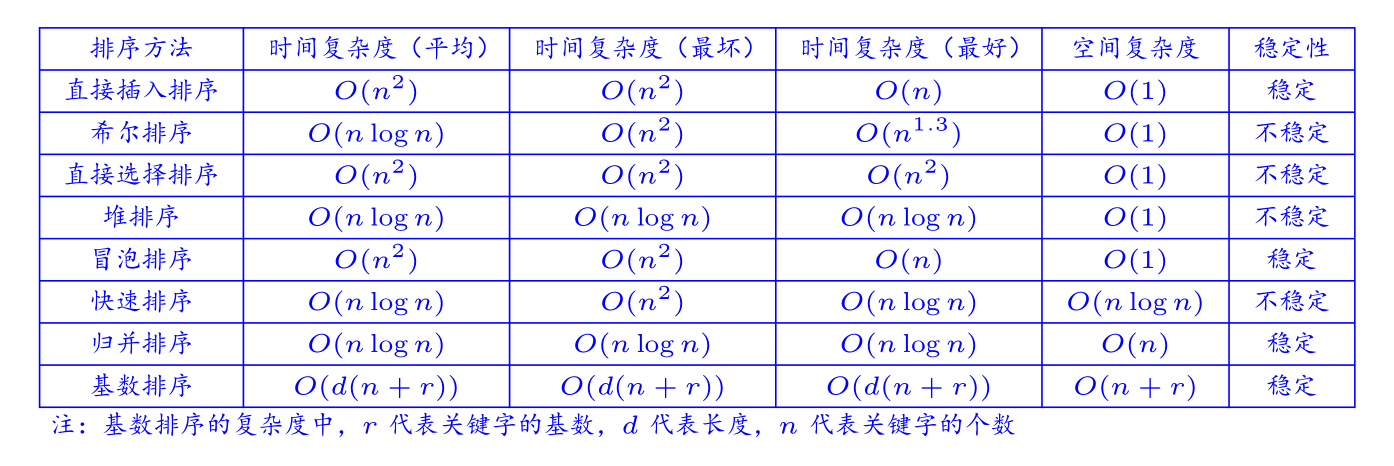
\includegraphics[scale=0.3]{day72.png}
\hfill\hphantom{~}
\end{tips}

\num 在\dm{java}中,下列对继承的说法,正确的是(~~~\textcolor[rgb]{1.00,0.00,0.00}{A}~~~)。

A.子类能继承父类所有的成员 \hfill B.子类继承父类的非私有方法和状态

C.子类只能继承父类的\dm{public}方法和状态 \hfill D.子类只能继承父类的方法

\begin{jie}
子类继承父类的全部,但只能使用非私有成员变量和方法。
\end{jie}

\num 给定一个非负的整数数组\dm{A},返回一个数组,在该数组中, \dm{A}的所有偶数元素之后跟着所有奇数元素。
\href{https://leetcode-cn.com/problems/sort-array-by-parity/} {OJ链接-按奇偶排序数组}

\begin{tips}
1.使用左指针指向数组的左侧,右指针指向数组的右侧

2.如果左指针指的是偶数,左指针向右移动,右指针指的是奇数,右指针向左移动

3.经过上一步,左指针指向为奇数,右指针指向的为偶数,交换这两个指针指的元素的值。

4.左指针在右指针的左侧时,重复第二步、第三部。
\end{tips}

\begin{lstlisting}[title=按奇偶排序数组]
class Solution {
    public int[] sortArrayByParity(int[] A) {
        int lo = 0;
        int hi = A.length - 1;
        while(lo < hi){
            if(A[lo] % 2 == 0){
                lo++;
            }
            if(A[hi] % 2 == 1){
                hi--;
            }
            if(lo < hi && A[lo] % 2 == 1 && A[hi] % 2 == 0){
                int tmp = A[lo];
                A[lo] = A[hi];
                A[hi] = tmp;
            }
        }
        return A;
    }
}
\end{lstlisting}

\num 给定一个整数类型的数组\dm{ nums},请编写一个能够返回数组 “中心索引” 的方法。

我们是这样定义数组 中心索引 的:数组中心索引的左侧所有元素相加的和等于右侧所有元素相加的和。

如果数组不存在中心索引,那么我们应该返回 -1。如果数组有多个中心索引,那么我们应该返回最靠近左边的那一个。\href{https://leetcode-cn.com/problems/find-pivot-index/} {OJ链接-寻找数组的中心索引}

\begin{tips}
1.计算出数组的和;

2.从左至右遍历数组,计算出第\dm{i}个元素左侧元素的和(包含该元素\dm{A[i]})\dm{sum1}和右侧元素的和(包含该元素\dm{A[i]})\dm{sum2},如果\dm{sum1}和\dm{sum2}相等,说明该位置为中心索引。

3.遍历完依旧没有符合题意的返回\dm{-1}。
\end{tips}

\begin{lstlisting}[title=寻找数组的中心索引]
class Solution {
    public int pivotIndex(int[] nums) {
        int sum1 = 0;
        for(int x : nums){
            sum1 += x;
        }
        int sum2 = 0;
        for(int i = 0; i < nums.length; i++){
            sum2 += nums[i];
            if(sum1 == sum2){
                return i;
            }
            sum1 = sum1 - nums[i];
        }
        return -1;
    }
}
\end{lstlisting}

\newpage
\section{}
\num (\textbf{多选题})已知\dm{boolean result = false},则下面哪个选项是合法的(~~\textcolor[rgb]{1.00,0.00,0.00}{B}、\textcolor[rgb]{1.00,0.00,0.00}{D}~~)。

A.\dm{result = 1} \hfill B.\dm{result = true}
\hfill
 C.\dm{if (result != 0) { }} \hfill D.\dm{if (result) { }}

 \begin{jie}
 \dm{boolean}类型不能和其他类型进行相互赋值、比较。
 \end{jie}

 \num (\textbf{多选题})下面的\dm{switch}语句中,\dm{x}可以是哪些类型的数据(~~\textcolor[rgb]{1.00,0.00,0.00}{B}、\textcolor[rgb]{1.00,0.00,0.00}{D}~~)。

\begin{lstlisting}[numbers=none]
switch(x){
    default:
    System.out.println("hello");
}
\end{lstlisting}

A.\dm{long}\hfill B.\dm{char}\hfill C.\dm{float}\hfill D.\dm{byte}\hfill E.\dm{double}\hfill F.\dm{Object}

\begin{tips}
\dm{switch}中支持的数据类型:\dm{char}、\dm{byte}、\dm{short}、\dm{int}、\dm{Character}、\dm{Byte}、\dm{Short}、\dm{Integer}、\dm{String}、\dm{char}、\dm{enum}。
\end{tips}

\num (\textbf{多选题})关于运行时常量池,下列那个说法是正确的(~\textcolor[rgb]{1.00,0.00,0.00}{B}、\textcolor[rgb]{1.00,0.00,0.00}{C}、\textcolor[rgb]{1.00,0.00,0.00}{D}~)。

A.运行时常量池大小受栈区大小的影响

B.运行时常量池大小受方法区大小的影响

C.存放了编译时期生成的各种字面量

D.存放编译时期生成的符号引用

\begin{tips}
运行时常量池是方法区的一部分。class文件中除了有类的版本、字段、方法、接口等描述信息外,还有一项信息是常量池,用于存放编译期生成的各种字面量和符号引用,这部分内容将在类加载后进入方法区的运行时常量池中存放。
\end{tips}

\num 给定一个由\textbf{整数}组成的 \textbf{非空} 数组所表示的非负整数,在该数的基础上加一。最高位数字存放在数组的首位, 数组中每个元素只存储单个数字。你可以假设除了整数 0 之外,这个整数不会以零开头。(第一个数字是9或者最后一个是9要考虑进位)\href{https://leetcode-cn.com/problems/plus-one/} {OJ链接-加一}

\begin{tips}
1.将数组的最后一个元素加一;

2.加一后只有两种情况,等于10或小于10.

3.等于10,将其除10取余即为该位的值,同时将指针前移一位,将前一位加一,然后重复3、4步;

4.小于10,不需要进位,直接返回。

5.对于9,99,999…这种加一后,长度增加的,直接创建一个比原数组长度长1的数组,将新数组首位初始化为1,其余保持不变(默认初始化为0)。
\end{tips}


\begin{lstlisting}[title=加一]
class Solution {
    public int[] plusOne(int[] digits) {
        for(int i = digits.length - 1; i >= 0; i--){
            digits[i]++;
            digits[i] = digits[i] % 10;
            if(digits[i] != 0){
                return digits;
            }
        }
        int[] arr = new int[digits.length + 1];
        arr[0] = 1;
        return arr;
    }
}
\end{lstlisting}

\num 给你一个非空数组,返回此数组中 第三大的数 。如果不存在,则返回数组中最大的数。\href{https://leetcode-cn.com/problems/third-maximum-number/} {OJ链接-第三大的数}

\begin{tips}
1.数组长度为1,直接返回该元素。

2.数组长度为2,返回两个中最大的那个。

3.数组长度大于等于3:

题目中数的范围为\dm{int}的范围,所以数组中第三大的元素可能是\dm{int}的最小值(\dm{Integer.MIN_VALUE})。

使用三个数\dm{max1}、\dm{max2}、\dm{max3}分别表示数组中第一大,第二大,第三大的元素,将其初始化为\dm{int}的最小值减一(即\dm{Integer.MIN_VALUE - 1},把这个值记为\dm{min}),因为超出了\dm{int}的范围,所以;类型为\dm{long}。

遍历数组,对于任意元素:

如果该元素大于\dm{max1},就把\dm{max2}的值赋给\dm{max3},把\dm{max1}的值赋给\dm{max2},把该元素的值赋给\dm{max1};

如果该元素等于\dm{max1},检查下一个元素,即\dm{continue};

如果该元素小于\dm{max1},则将该元素与\dm{max2}比较:

如果该元素大于\dm{max2},就把\dm{max2}的值赋给\dm{max3},把该元素的值赋给\dm{max2};

如果该元素等于\dm{max2},检查下一个元素,即\dm{continue};

如果该元素小于\dm{max2},则将该元素与\dm{max3}比较:

只有该元素大于\dm{max3}时,才将该元素的值赋给\dm{max3},否则不操作。

遍历完数组后,看\dm{max3}的值是否为\dm{min},如果是,说明没有第3大的数,返回\dm{max1},否则返回\dm{max3}。因为其类型为\dm{long},还需要进行类型转换。
\end{tips}

\begin{lstlisting}[title=第三大的数]
class Solution {
    public int thirdMax(int[] nums) {
        if(nums.length == 1){
            return nums[0];
        }
        if(nums.length == 2){
            return nums[0] > nums[1] ? nums[0] : nums[1];
        }
        long min = (long)Integer.MIN_VALUE - 1;
        long max1 = min;
        long max2 = max1;
        long max3 = max2;

        for(int i = 0; i < nums.length; i++){
            if(nums[i] > max1){
                max3 = max2;
                max2 = max1;
                max1 = nums[i];
            }else if(nums[i] == max1) {
                continue;
            }else{
                if(nums[i] > max2){
                    max3 = max2;
                    max2 = nums[i];
                }else if(nums[i] == max2){
                    continue;
                }else{
                    if(nums[i] > max3){
                        max3 = nums[i];
                    }
                }
            }
        }
        return max3 == min ? (int)max1 : (int)max3;
    }
}
\end{lstlisting}
\newpage
\section{}
\num 下列类定义中哪些是合法的抽象类的定义(~~~\textcolor[rgb]{1.00,0.00,0.00}{C}~~~)。

A.\dm{abstract Animal{abstract void growl();}}

B.\dm{class abstract Animal{abstract void growl();}}

C.\dm{abstract class Animal{abstract void growl();}}

D.\dm{abstract class Animal{abstract void growl(){System.out.println( “growl”);};}}

\begin{tips}
定义类使用\dm{class}关键字,该关键字与类名紧邻,中间不能有其他关键字或符号。

抽象方法不能有方法体。
\end{tips}

\num 在\dm{java}中,无论在何处调用,使用静态属性必须以类名做前缀。(~~~\textcolor[rgb]{1.00,0.00,0.00}{B}~~~)

A.正确\hfill B.错误\hfill\hphantom{B.错误}\hfill\hphantom{B.错误}

\begin{jie}
可以使用对象名来调用静态属性,但其本质上是通过对象找到其对应的类,然后调用该静态属性。
\end{jie}

\num 哪个关键字可以对对象加互斥锁(~~~\textcolor[rgb]{1.00,0.00,0.00}{A}~~~)。

A.\dm{synchronized} B.\dm{volatile} C.\dm{serialize} D.\dm{ static}

\begin{tips}
\dm{synchronized}:用来给对象和方法或者代码块加锁. 当它锁定一个方法或者一个代码块的时候, 同一时刻最多只有一个线程执行这个段代码。

\dm{volatile}:用来确保将变量的更新操作通知到其他线程, 当把变量声明为\dm{volatile}类型后, 编译器与运行时都会注意到这个变量是共享的, 因此不会将该变量上的操作与其他内存操作一起重排序. 然而, 在访问\dm{volatile}变量时, 不会执行加锁操作, 因此也就不会使执行线程阻塞, 因此, \dm{volatile}变量是一种比\dm{synchronized}关键字更轻量级的同步机制。

\dm{serialize}:Java对象序列化为二进制文件。

\dm{static}:修饰类变量、类方法,静态代码块。
\end{tips}

\num 给定一个整数数组 nums 和一个整数目标值 target,请你在该数组中找出 和为目标值 的那 两个 整数,并返回它们的数组下标。
你可以假设每种输入只会对应一个答案。但是,数组中同一个元素不能使用两遍。
你可以按任意顺序返回答案。要求时间复杂度$O(n)$,当然也可以选择使用暴力的$O(n^2)$的解法。\href{https://leetcode-cn.com/problems/two-sum/} {OJ链接-两数之和}

\begin{tips}
1.从左至右遍历数组。

2.一个指针指向当前元素,另一个指针从当前元素的下一位至数组最后遍历,寻找与当前元素的和等于目标值的元素。找到后返回这两个指针对应的下标值。
\end{tips}

\begin{lstlisting}[title=两数之和]
class Solution {
    public int[] twoSum(int[] nums, int target) {
        for(int i = 0; i< nums.length;i++){
            for(int j = i + 1;j < nums.length;j++){
                if(nums[j] == target - nums[i]){
                    int[] ret = {i,j};
                    return ret;
                }
            }
        }
        return new int[0];
    }
}
\end{lstlisting}

\num 给你两个二进制字符串,返回它们的和(用二进制表示)。
输入为 \textbf{非空} 字符串且只包含数字 \dm{1} 和 \dm{0}。\href{https://leetcode-cn.com/problems/add-binary/} {OJ链接-二进制求和}

\begin{tips}
1.首先将短的字符串用0将高位补齐。因为要对字符频繁的操作,所以使用可变字符序列对象\dm{StringBuilder}。可以先将题中的两个字符串翻转,在最短的字符串后补0(使用\dm{append}方法),最后计算结束再将字符串翻转。

2.字符串补齐后,使用列竖式的方法计算每一位,用\dm{carry}来表示进位,刚开始进位为0,。

3.获取每一位的字符,因为只有0和1,所以减去字符0即为数字0和1。每一位的和为\dm{carry + a对应位置的值 + b对应位置的值},记为\dm{count},因为是2进制,所以\dm{count}大于等于2时,要进行进位,即\dm{carry}置为1,同时该位置的\dm{count\%2}。

4.计算结束后,要判断\dm{carry}的值,如果这个值是1,说明还需要进一位。

5.别忘了翻转和返回值的类型。
\end{tips}

\begin{lstlisting}[title=二进制求和]
class Solution {
    public String addBinary(String a, String b) {
        //求两个字符串的长度
        int a1 = a.length();
        int b1 = b.length();
        //求字符串的最大长度
        int max = a1 >= b1 ? a1 : b1;
        //将字符串存入可变字符序列并进行翻转
        StringBuilder stringBuilder1 = new StringBuilder(a).reverse();
        StringBuilder stringBuilder2 = new StringBuilder(b).reverse();
        //对短字符串进行补0
        while(stringBuilder1.length() < max){
            stringBuilder1.append("0");
        }
        while(stringBuilder2.length() < max){
            stringBuilder2.append("0");
        }
        //进位,初始为0
        int carry = 0;

        int x = 0;
        int y = 0;
        int count = 0;
        //存放相加的结果
        StringBuilder ret = new StringBuilder();
        for(int i = 0; i < max; i++){
            x = stringBuilder1.charAt(i) - '0';
            y = stringBuilder2.charAt(i) - '0';
            //每一位结果等于进位加各数
            count = x + y + carry;
            //二进制,结果超过2,就需要进位
            if(count >= 2){
                carry = 1;
                ret.append(count % 2);
            }else{
                carry = 0;
                ret.append(count);
            }
        }
        //最高位的进位判断
        if(carry == 1){
            ret.append("1");
        }
        //别忘了翻转,注意方法的返回类型
        return ret.reverse().toString();
    }
}
\end{lstlisting}

\newpage
\section{}
\num 一个Java源程序文件中定义几个类和接口,则编译该文件后生成几个以.class为后缀的字节码文件。(~~~\textcolor[rgb]{1.00,0.00,0.00}{A}~~~)

A.正确\hfill B.错误\hfill\hphantom{B.错误}\hfill\hphantom{B.错误}

\num 要使某个类能被同一个包中的其他类访问,但不能被这个包以外的类访问,可以(~~~\textcolor[rgb]{1.00,0.00,0.00}{A}~~~)。

A.让该类不使用任何关键字

B.使用\dm{private} 关键字

C.使用\dm{protected} 关键字

D.使用\dm{void}关键字

\begin{tips}
不使用关键字:包访问权限,即只能同包的类访问。

\dm{private}:类访问权限,只能在类的内部访问,出了类则无法访问。

\dm{protected}:同包的类可以访问,不通包的子类也可以访问。

\dm{public}:任意包中的类都可以访问。

\dm{void}:方法的返回类型,与访问权限无关。
\end{tips}

\num 判断对错。在java的多态调用中,new的是哪一个类就是调用的哪个类的方法。(~~~\textcolor[rgb]{1.00,0.00,0.00}{A}~~~)

A.正确\hfill B.错误\hfill\hphantom{B.错误}\hfill\hphantom{B.错误}

\num 字符串转换函数\href{https://leetcode-cn.com/problems/string-to-integer-atoi/} {OJ链接-字符串转换整数atoi}。

请你来实现一个\dm{myAtoi(string s)}函数,使其能将字符串转换成一个 32 位有符号整数(类似\dm{C/C++}中的\dm{atoi}函数)。

函数\dm{myAtoi(string s)}的算法如下:
\begin{itemize}
\itemsep=0pt \parskip=0pt%删除排序列表之间的垂直空白
  \item 读入字符串并丢弃无用的前导空格。
  \item 检查第一个字符(假设还未到字符末尾)为正还是负号,读取该字符(如果有)。 确定最终结果是负数还是正数。 如果两者都不存在,则假定结果为正。
  \item 读入下一个字符,直到到达下一个非数字字符或到达输入的结尾。字符串的其余部分将被忽略。
  \item 将前面步骤读入的这些数字转换为整数(即,"123" $\rightarrow$ 123, "0032" $\rightarrow$32)。如果没有读入数字,则整数为 0 。必要时更改符号(从步骤 2 开始)。
  \item 如果整数数超过 32 位有符号整数范围$[−2^{31},  2^{31} − 1]$ ,需要截断这个整数,使其保持在这个范围内。具体来说,小于$−2^{31}$ 的整数应该被固定为$−2^{31}$ ,大于$2^{31} − 1$的整数应该被固定为$2^{31} − 1$。
\item 返回整数作为最终结果。
\end{itemize}

\textbf{注意}:
\begin{itemize}
\itemsep=0pt \parskip=0pt
\item 本题中的空白字符只包括空格字符\dm{' '} 。
\item 除前导空格或数字后的其余字符串外,请勿忽略 任何其他字符。
\end{itemize}

\begin{tips}
1.对于空字符串和\dm{null},直接返回0;

2.一般字符串:

依题意,首先扫描空格,当指针没有到达末尾且指向的字符为空格时,指针向右移动。

空格扫描完后,判断指针是否到达末尾,如果到达末尾,返回0.

没有到达末尾,扫描下一个字符是否是\dm{+}或\dm{-},使用\dm{flag}作为正负的标记(默认为1),若扫描到\dm{+},\dm{flag}不变,指针向后移动一位。若扫描到\dm{1},\dm{flag}置为\dm{-1},指针向后移动一位。

再次判断是否到达末尾,如果到达末尾,返回0.

没有到达末尾,继续扫描:(使用\dm{ret}存储扫描的数字,因为数字可能超过\dm{int}的最大范围,所以\dm{ret}为\dm{long}类型)

如果是数字,将其放到\dm{ret}的后边,即\dm{ret = ret * 10},然后判断\dm{ret}的大小,如果\dm{flag}为1,且\dm{ret}超过整型的最大值,则返回\dm{Integer.MAX_VALUE},如果\dm{flag}为-1,且\dm{-ret}小于整型的最小值,则返回\dm{Integer.MIN_VALUE}。

如果不是数字或者指针已经扫描到了末尾,退出循环。

如果\dm{ret}没有超过整型的范围,返回\dm{flag * ret}。要注意类型的转换。
\end{tips}

\begin{lstlisting}[title=字符串转换整数atoi]
class Solution {
    public int myAtoi(String s) {
        if(s == null || s.length() == 0){
            return 0;
        }
        int i = 0;
        long ret = 0;
        int flag = 1;
        while(i < s.length() && s.charAt(i) == ' '){
            ++i;
        }
        if(i >= s.length()){
            return 0;
        }
        if(s.charAt(i) == '-'){
            flag = -1;
            i++;
        }else if(s.charAt(i) == '+'){
            i++;
        }

        if(i >= s.length()){
            return 0;
        }

        while(i < s.length() && (s.charAt(i) >= '0' && s.charAt(i) <= '9')){
            int x = s.charAt(i) - '0';
            ret = ret * 10 + x;
            if(flag > 0 && ret > Integer.MAX_VALUE){
                return Integer.MAX_VALUE;
            }
            if(flag < 0 && -ret < Integer.MIN_VALUE){
                return Integer.MIN_VALUE;
            }
            ++i;
        }
        return flag > 0 ? (int)ret : -(int)ret;
    }
}
\end{lstlisting}

\num 给定一个按照升序排列的整数数组\dm{nums},和一个目标值 \dm{target}。找出给定目标值在数组中的开始位置和结束位置。
如果数组中不存在目标值\dm{target},返回 $[-1, -1]$。
\href{https://leetcode-cn.com/problems/find-first-and-last-position-of-element-in-sorted-array/} {OJ链接-在排序数组中查找元素的第一个和最后一个位置}。

\begin{tips}
使用二分查找。

关键在于等于时的情况处理:

寻找下界:如果\dm{mid}处的值等于目标值,判断\dm{mid}的左侧值是否等于目标值,如果左侧没有值或者左侧不等于目标值,说明该\dm{mid}为下界,否则需要从\dm{[lo,mid - 1]}区间来查找下界,即\dm{hi = mid - 1}

寻找上界:与寻找下界逻辑相反,如果\dm{mid}处的值等于目标值,判断\dm{mid}的右侧值是否等于目标值,如果右侧没有值或者右侧不等于目标值,说明该\dm{mid}为上界,否则需要从\dm{[mid + 1, hi]}区间来查找上界,即\dm{lo = mid + 1}
\end{tips}

\begin{lstlisting}[title=在排序数组中查找元素的第一个和最后一个位置]
class Solution {
    private int findFirst(int[] nums, int target) {
        int lo = 0;
        int hi = nums.length - 1;
        int mid = 0;
        while(lo <= hi){
            mid = lo + ((hi - lo) >> 1);
            if(nums[mid] < target){
                lo = mid + 1;
            }else if(target < nums[mid]){
                hi = mid - 1;
            }else{
                if(mid == 0 || nums[mid - 1] != target){
                    return mid;
                }else{
                    hi = mid - 1;
                }
            }
        }
        return -1;
    }

    private int findLast(int[] nums, int target) {
        int lo = 0;
        int hi = nums.length - 1;
        int mid = 0;
        while(lo <= hi){
            mid = lo + ((hi - lo) >> 1);
            if(nums[mid] < target){
                lo = mid + 1;
            }else if(target < nums[mid]){
                hi = mid - 1;
            }else{
                if(mid == nums.length - 1 || nums[mid + 1] != target){
                    return mid;
                }else{
                    lo = mid + 1;
                }
            }
        }
        return -1;
    }
    public int[] searchRange(int[] nums, int target) {
        return new int[]{findFirst(nums,target),findLast(nums,target)};

    }
}
\end{lstlisting}

\newpage
\section{}
\num 执行下列代码的输出结果是(~~~\textcolor[rgb]{1.00,0.00,0.00}{C}~~~)。
\begin{lstlisting}
public class Demo{
    public static void main(String args[]){
        int num = 10;
        System.out.println(test(num));
    }
    public static int test(int b){
        try {
            b += 10;
            return b;
        }catch(RuntimeException e){

        }catch(Exception e2){

        }finally{
            b += 10;
            return b;
        }
    }
}
\end{lstlisting}

A.\dm{10}\hfill  B.\dm{20}\hfill C.\dm{30}\hfill D.\dm{40}

\begin{tips}
如果有\dm{finally}语句,在\dm{try}和\dm{catch}中遇到\dm{return},先执行\dm{finally}中的语句,如果在\dm{finally}中遇到了\dm{return},则直接返回,如果\dm{finally}中没有\dm{return}语句,则返回至\dm{try}或\dm{catch}中的\dm{return}处。
\end{tips}

\num 下面关于Java package的描述,哪个是正确的(~~~\textcolor[rgb]{1.00,0.00,0.00}{B}~~~)。

\myroman{1}.包不提供将所有类名分区为更易管理的块的机制。

\myroman{2}.包提供可见性控制机制。

\myroman{3}.	包的一个重要属性是包内定义的所有类都可以通过该包外的代码访问。

\myroman{4}.	声明为包的一部分的类的.class文件可以存储在多个目录中.

A.只有\myroman{1}\hfill B.只有\myroman{2}\hfill C.只有\myroman{3}\hfill D.只有\myroman{4}

\begin{tips}
为了更好地组织类,Java 提供了包机制,用于区别类名的命名空间。

包的作用
1、把功能相似或相关的类或接口组织在同一个包中,方便类的查找和使用。

2、如同文件夹一样,包也采用了树形目录的存储方式。同一个包中的类名字是不同的,不同的包中的类的名字是可以相同的,当同时调用两个不同包中相同类名的类时,应该加上包名加以区别。因此,包可以避免名字冲突。

3、包也限定了访问权限,拥有包访问权限的类才能访问某个包中的类。

Java 使用包(package)这种机制是为了防止命名冲突,访问控制,提供搜索和定位类(class)、接口、枚举(enumerations)和注释(annotation)等。
\end{tips}

\num Java数据库连接库JDBC用到哪种设计模式(~~~\textcolor[rgb]{1.00,0.00,0.00}{B}~~~)。

A.生成器\hfill B.桥接模式\hfill C.抽象工厂\hfill D.单例模式

\num 给定一个字符串,验证它是否是回文串,只考虑字母和数字字符,可以忽略字母的大小写。

说明:本题中,我们将空字符串定义为有效的回文串。
\href{https://leetcode-cn.com/problems/valid-palindrome/}{OJ链接-验证回文串}

\begin{tips}
1.处理空字符串:是回文串

2.只关注字母和数字,所以写一个私有方法来判断当前字符是否为字母/数字。

3.使用左右指针指向字符串的开头和结尾。

4.如果不是字母或数字,左指针右移,右指针左移。

5.经过上一后左右指针指向的字符则为字母或数字。题目中不区分大小写,所以如果字符是大写字母,将其转换为小写字母(也可以把小写的字符转为大写的)。

6.因为字符串是不可变对象,所以使用字符来接收左右指针指向的字符,大写字符转小写:\dm{ch - 'A' + 'a'},字符相加减本质上是其对应的\dm{ASCII}码相加减,因此还需将其强制转换为字符。

7.大写转为小写后,比较两个字符是否相等,如果不相等,返回\dm{false}。如果相等,左指针左移,右指针右移。继续第5到第7步。

8.若左指针和右指针重合,说明是回文串。
\end{tips}

\begin{lstlisting}[title=验证回文串]
class Solution {
    private boolean isAlphaAndNum(char ch){
        if((ch >= 'a' && ch <= 'z') || (ch >= 'A' && ch <= 'Z') || (ch >= '0' && ch <= '9')){
            return true;
        }
        return false;
    }
    public boolean isPalindrome(String s) {
        if(s == null || " ".equals(s)){
            return true;
        }
        int lo = 0;
        int hi = s.length() - 1;
        char a;
        char b;
        while(lo < hi){
            if(!isAlphaAndNum(s.charAt(lo))){
                lo++;
            }
            if(!isAlphaAndNum(s.charAt(hi))){
                hi--;
            }
            if(lo < hi && isAlphaAndNum(s.charAt(lo)) && isAlphaAndNum(s.charAt(hi))){
                a = s.charAt(lo);
                b = s.charAt(hi);
                if(a >= 'A' && a <= 'Z'){
                    a = (char)(a + 'a' - 'A');
                }
                if(b >= 'A' && b <= 'Z'){
                    b = (char)(b + 'a' - 'A');
                }
                if(a != b){
                    return false;
                }
                lo++;
                hi--;
            }
        }
        return true;
    }
}
\end{lstlisting}

\num 给定一组字符,使用\textcolor[rgb]{0.00,1.00,0.25}{原地算法}将其压缩。压缩后的长度必须始终小于或等于原数组长度。数组的每个元素应该是长度为1 的字符(不是\dm{int}整数类型)。在完成原地修改输入数组后,返回数组的新长度。\href{https://leetcode-cn.com/problems/string-compression/}{OJ链接-压缩字符串}

\begin{tips}
使用三个指针。

1.指针\dm{i}指向开头。第三个指针\dm{index}从头开始。

2.\dm{j}指向\dm{i}的下一个位置。

3.如果指针\dm{j}指向的字符等于指针\dm{i}指向的字符,指针\dm{j}向后移动,直到与指针\dm{i}指向的字符不相等(或者到字符串的末尾)停下来。

4.两种情况:\\
a.若\dm{j}在\dm{i}下一位停下来,表示\dm{i}指向的字符只有一个,不需要压缩,此时\dm{j - i}为1。\\
b.若\dm{j}在\dm{i}的后边位置停下来(超过1位),假设\dm{i}为0,\dm{j}为4,说明位置\dm{0、1、2、3}的字符都相等,即有连续\dm{j - i}个字符相等。

5.在\dm{index}处记录\dm{i}处的字符,然后向右移动一位,如果\dm{j - i}为1,不需要压缩,如果\dm{j - i}大于1,题目给的字符数组的长度最大为1000,可能出现连续字符个数最大为1000,即\dm{j - i}超过一位数,把该数转换为字符数组,然后把数的每一位依次填入\dm{index}处(填一位\dm{index}向右移动一位)(代码的12-15行)。

6.上一步执行完后,将指针\dm{i}移到指针\dm{j}处,执行2-5步,直到全部字符串扫描结束。
\end{tips}

\begin{lstlisting}[title=压缩字符串]
class Solution {
    public int compress(char[] chars) {
        int index = 0;
        int i = 0;
        int j = 1;
        while(i < chars.length && index < chars.length){
            while(j < chars.length && chars[j] == chars[i]){
                j++;
            }
            chars[index++] = chars[i];
            int sum = j - i;
            if(sum > 1 && index < chars.length){
                for(char ch : ("" + sum).toCharArray()){
                    chars[index++] = ch;
                }
            }
            i = j;
            j = i + 1;
        }
        return index;
    }
}
\end{lstlisting}
\newpage
\section{}
\num 下列哪个选项是正确计算$42°$(角度)的余弦值(~~~\textcolor[rgb]{1.00,0.00,0.00}{C}~~~)。

A.\dm{double d=Math.cos(42)}

B.\dm{double d=Math.cosine(42)}

C.\dm{double d=Math.cos(Math.toRadians(42))}

D\dm{double d=Math.cos(Math.toDegrees(42))}

\begin{tips}
\dm{Math.toDegrees()}用于将\dm{()}中的参数转化为角度。

\dm{Math.toDegrees()}用于将\dm{()}中的参数转化为弧度。

\dm{Math.cos()}中的参数为弧度。

计算$42°$(角度)的余弦值:把$42°$转化为弧度,然后求余弦。
\end{tips}

\num \dm{String s = new String("xyz")}创建了几个\dm{String}对象(~~~\textcolor[rgb]{1.00,0.00,0.00}{C}~~~)。

A.两个或一个都有可能\hfill B.两个\hfill  C.一个\hfill  D.三个

\num 下列代码输出结果为(\hphantom{~~~~~})。

A.

动物可以移动

狗可以跑和走

狗可以吠叫

B.
动物可以移动 动物可以移动 狗可以吠叫

C.运行错误

D.编译错误

\begin{jie}
没有代码。
\end{jie}

\num 给你一个整数数组\dm{nums},你需要找出一个\textbf{连续子数组},如果对这个子数组进行升序排序,那么整个数组都会变为升序排序。请你找出符合题意的 最短 子数组,并输出它的长度。\href{https://leetcode-cn.com/problems/shortest-unsorted-continuous-subarray/} {OJ链接-最短无序连续子数组}
\begin{lstlisting}[title=最短无序连续子数组]
class Solution {
    public int findUnsortedSubarray(int[] nums) {

    }
}
\end{lstlisting}

\num 根据\textbf{逆波兰表示法},求表达式的值。
有效的运算符包括\dm{+},\dm{-},\dm{*},\dm{/} 。每个运算对象可以是整数,也可以是另一个逆波兰表达式。\href{https://leetcode-cn.com/problems/evaluate-reverse-polish-notation/} {OJ链接-逆波兰表达式求值}

\textbf{说明}:
\begin{itemize}
\itemsep=0pt \parskip=0pt
  \item 整数除法只保留整数部分。
  \item 给定逆波兰表达式总是有效的。换句话说,表达式总会得出有效数值且不存在除数为 0 的情况。
\end{itemize}

\begin{lstlisting}[title=逆波兰表达式求值]
class Solution {
    public int evalRPN(String[] tokens) {

    }
}
\end{lstlisting}

\newpage
\section{}
\num (\textbf{多选题})关于\dm{Java}以下描述正确的有(\hphantom{~~~~~})。

A.\dm{Class}类是\dm{Object}类的超类\hfil  B.\dm{Object}类是一个\dm{final}类

C.\dm{String}类是一个\dm{final}类
\hfill D.\dm{Class}类可以装载其它类

\num (\textbf{多选题})\dm{Java}中的集合类包括\dm{ArrayList}、\dm{LinkedList} 、\dm{HashMap}等类,下列关于集合类描述正确的是(\hphantom{~~~~~})。

A.\dm{ArrayList}和\dm{LinkedList}均实现了\dm{List}接口

B.\dm{ArrayList}的访问速度比\dm{LinkedList}快

C.添加和删除元素时,\dm{ArrayList}的表现更佳

D.\dm{HashMap}实现\dm{Map}接口,它允许任何类型的键和值对象,并允许将\dm{null}用作键或值

\num (\textbf{多选题})关于\dm{equals}和\dm{hashCode}描述正确的是 (\hphantom{~~~~~})。

A.两个\dm{obj},如果\dm{equals()}相等,\dm{hashCode()}一定相等(符合代码规范的情况下)

B.两个\dm{obj},如果\dm{hashCode()}相等,\dm{equals()}不一定相等

C.两个不同的\dm{obj},\dm{hashCode()}可能相等

D.其他都不对

\num 给你一个整数数组 nums ,数组中的元素\CJKunderdot{互不相同}。返回该数组所有可能的子集(幂集)。
解集\CJKunderdot{不能}包含重复的子集。你可以按\CJKunderdot{任意顺序}返回解集。
\href{https://leetcode-cn.com/problems/subsets/} {OJ链接-子集}

\begin{lstlisting}[title=子集]
class Solution {
    public List<List<Integer>> subsets(int[] nums) {

    }
}
\end{lstlisting}

\num 给定一个整数矩阵,找出最长递增路径的长度。
对于每个单元格,你可以往上,下,左,右四个方向移动。 你不能在对角线方向上移动或移动到边界外(即不允许环绕)。
\href{https://leetcode-cn.com/problems/longest-increasing-path-in-a-matrix/} {OJ链接-矩阵中最长递增路径}

\begin{lstlisting}[title=矩阵中最长递增路径]
class Solution {
    public int longestIncreasingPath(int[][] matrix) {

    }
}
\end{lstlisting}

\newpage
\section{}
\num (\textbf{多选题})下面有关\dm{java}的\dm{instanceof}、 \dm{?}、\dm{&} 、\dm{&&}说法正确的有(\hphantom{~~~~~})。

A.\dm{instanceof}可用来判断某个实例变量是否属于某种类的类型。

B.\dm{"? :" }三目运算符

C.\dm{&}在逻辑运算中是非短路逻辑与,在位运算中是按位与

D.\dm{&&}逻辑运算:逻辑与

\num (\textbf{多选题})下面哪个语句是创建数组的正确语句?(\hphantom{~~~~~})。

A.\dm{float f[][] = new float[6][6]; }

B.\dm{float []f[] = new float[6][6];}

C.\dm{float f[][] = new float[][6];}

D.\dm{float [][]f = new float[6][6];}

E.\dm{float [][]f = new float[6][];}

\num 下列类在多重\dm{catch}中同时出现时,哪一个异常类应最后一个列出(\hphantom{~~~~~})。

A.\dm{ArithmeticException }\hfill
B.\dm{NumberFormatException}\hfill
C.\dm{Exception}\hfill
D.\dm{ArrayIndexOutOfBoundException}

\num 给定一棵二叉树,想象自己站在它的右侧,按照从顶部到底部的顺序,返回从右侧所能看到的节点值。\href{https://leetcode-cn.com/problems/binary-tree-right-side-view/} {OJ链接-二叉树的右视图}

\begin{lstlisting}[title=二叉树的右视图]
/**
 * Definition for a binary tree node.
 * public class TreeNode {
 *     int val;
 *     TreeNode left;
 *     TreeNode right;
 *     TreeNode() {}
 *     TreeNode(int val) { this.val = val; }
 *     TreeNode(int val, TreeNode left, TreeNode right) {
 *         this.val = val;
 *         this.left = left;
 *         this.right = right;
 *     }
 * }
 */
class Solution {
    public List<Integer> rightSideView(TreeNode root) {

    }
}
\end{lstlisting}

\num 公交路线。\href{https://leetcode-cn.com/problems/bus-routes/} {OJ链接-公交路线}

我们有一系列公交路线。每一条路线\dm{routes[i]}上都有一辆公交车在上面循环行驶。例如,有一条路线\\ \dm{routes[0] = [1, 5, 7]},表示第一辆 (下标为0) 公交车会一直按照 $1\rightarrow 5\rightarrow 7\rightarrow 1\rightarrow 5\rightarrow 7\rightarrow 1\rightarrow \ldots $的车站路线行驶。

假设我们从$S$车站开始(初始时不在公交车上),要去往$T$站。 期间仅可乘坐公交车,求出最少乘坐的公交车数量。返回$1-$表示不可能到达终点车站。

\begin{lstlisting}[title=公交路线]
class Solution {
    public int numBusesToDestination(int[][] routes, int S, int T) {

    }
}
\end{lstlisting}

\num 通配符匹配。\href{https://leetcode-cn.com/problems/wildcard-matching/} {OJ链接-通配符匹配}

给定一个字符串($s$)和一个字符模式 ($p$),实现一个支持\dm{ '?'} 和\dm{'*'}的通配符匹配。
\begin{itemize}
\itemsep=0pt \parskip=0pt
\item \dm{'?'}可以匹配任何单个字符。
\item \dm{'*'}可以匹配任意字符串(包括空字符串)。
\end{itemize}
两个字符串完全匹配才算匹配成功。

\textbf{说明}:
\begin{itemize}
\itemsep=0pt \parskip=0pt
\item $s$可能为空,且只包含从 \dm{a-z}的小写字母。
\item $s$可能为空,且只包含从 \dm{a-z}的小写字母,以及字符\dm{?}和\dm{*}。
\end{itemize}
\begin{lstlisting}[title=通配符匹配]
class Solution {
    public boolean isMatch(String s, String p) {

    }
}
\end{lstlisting}
\end{document}


